\section{Study Design}

In order to investigate whether amplitude or spatially based electrotactile feedback aids prosthetic control the most when removing the visual dependency, an experiment was set up. A feedback coding scheme based on spatial activation and a feedback scheme based on amplitude modulation was developed and will be presented later in \secref{sec:feed}. \\
XX\fxnote{This will be added when final subject has been tested} subjects were recruited, where the order of which feedback scheme the subjects would be trained/tested in was randomized. However, an equal number of subjects was assigned to each order. An overview of the subject population and demographics can be seen in \tabref{tab:demo}. 

{\small 
\begin{table}[H]
	\caption{Overview of subject population and demographics.}\label{tab:demo}
	\begin{tabular}{llll} \hline
		& \textbf{Age, mean(std)} & \multicolumn{2}{c}{\textbf{Gender n(\%)}} \\ \cline{3-4}
		&                & Female          & Male           \\ \hline
		\begin{tabular}[c]{@{}l@{}}\textbf{Total}\\ (n = X)\end{tabular}   & \multicolumn{1}{c}{X(X)}    & X(X)       & X(X)      \\
		\begin{tabular}[c]{@{}l@{}}\textbf{Order 1}\\ (n = X)\end{tabular} & \multicolumn{1}{c}{X(X)}    & X(X)       & X(X)      \\
		\begin{tabular}[c]{@{}l@{}}\textbf{Order 2}\\ (n = X)\end{tabular}    & \multicolumn{1}{c}{X(X)}    & X(X)       & X(X)      \\ \hline
	\end{tabular}
\end{table}
}
\vspace{-0.5cm}
Prior to enrollment, the subjects were assessed to meet the inclusion criteria stated in the experimental protocol, which can be found in \secref{Ex_protocol}. The subjects were handed an experiment introduction letter prior to the experiment session, which gave an introduction to the background of the study and the different task the subjects would have to go through. Upon enrollment, the subjects were asked to sign an informed consent form, which stated that the subjects had received adequate information about the experiment and that they were always able to withdraw from the experiment. The experiment was ethically approved by the ethic commitee of Region Nordjylland, Denmark (Approval number N-20150075).\\
The experiment was designed such that each subject was trained and tested in using both feedback schemes along with control during a single session experiment. A graphical illustration of the main stages that the subject went through can be seen in \figref{fig:std}. For all subjects data used to build the prosthetic motor control system was acquired first. Secondly, the subjects were given time to familiarize with the control system and subsequently, the achieved control was assessed through a target reaching test. Next, sensory thresholds used for feedback were determined for the subject. Subjects assigned to order 1 went through four steps of training and test using scheme 1 followed by the same four steps using scheme 2. Subjects assigned to order 2 went through the schemes in opposite order. The next sections will further document the implementation and execution of the experiment.     

\begin{figure}[H]                 
	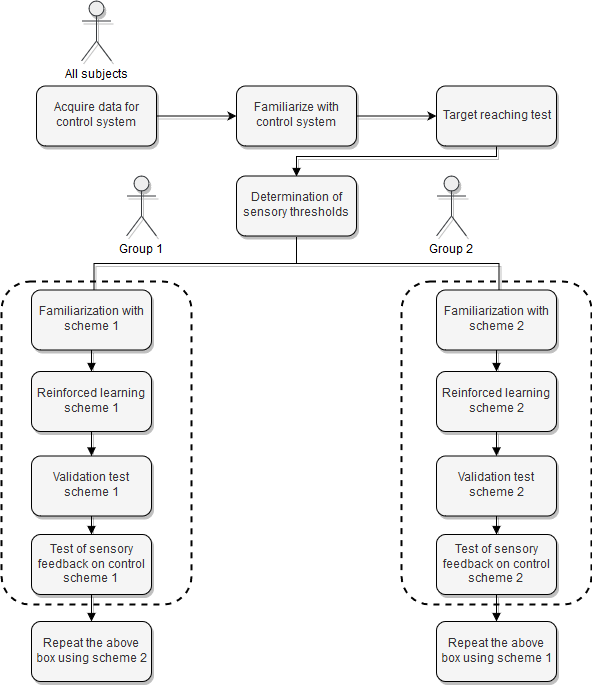
\includegraphics[width=.65\textwidth]{figures/std_design}
	\caption{Pipeline showing the stages of the experiment. Firstly, the stages common for all subjects were carried out followed by the order dependent stages. Scheme 1 was the spatially based and scheme 2 was the amplitude based.}
	\label{fig:std} 
\end{figure}